\documentclass{beamer}
\usepackage{natbib}
\usepackage{graphicx}
\title[MLRG: Bayes. Net. Complexity]{MLRG: The Computational Complexity of Probabilistic Inference Using Bayesian Belief Networks}
\author[Kui Tang]{Presented by Kui Tang}
\date{20 June 2012}
\usetheme{PaloAlto}
\usecolortheme{default}
\begin{document}

\frame{\titlepage}
\section{Background}
\begin{frame}
\frametitle{Bayesian belief networks are essential modelling tools}
\begin{itemize}
  \item Express densities functions of the form $$p(\mathbf{x}) = \prod_{i=1}^n p(x_i | \pi_i)$$ where $\pi_i$ denotes the parents of $x_i$ in the graph.
  \item Also called \emph{graphical models}, \emph{causal networks}
  \item Concisely express probabilistic models%%~\citep{bishop06}
  \begin{itemize}
    \item Visualize, design, and motivate new models.
    \item Simplify analysis and insight.
  \end{itemize}
  \item Examples: HMMs, Kalman filters, medical diagnoses.
  \item Sum-product algorithm provides exact inference for discrete and Gaussian trees.
  \item Other distributions can be computed by MCMC.
\end{itemize}
\end{frame}

\begin{frame}
\frametitle{A Bayesian belief network}
\includegraphics[width = \textwidth]{bayesnet}
\end{frame}

\begin{frame}
\frametitle{Inference in general discrete graphs is NP-complete.}
\begin{itemize}
  \item Definition: \emph{inference} in a belief network means calculating $p(S_1 | S_2)$ where $S_1$ and $S_2$ are two sets of variables.
  \begin{itemize}
    \item Example: $p(u_1 = T | Y = F, u_2 = T)$.
  \end{itemize}
  \item The \emph{most restricted form} of inference is computing $p(Y = T)$.
  \item If we show this form of inference is NP-hard, then all other forms of inference are also NP-hard. (Why?)
\end{itemize}
\end{frame}

\begin{frame}
\frametitle{Reduce from 3SAT}
\begin{centering}
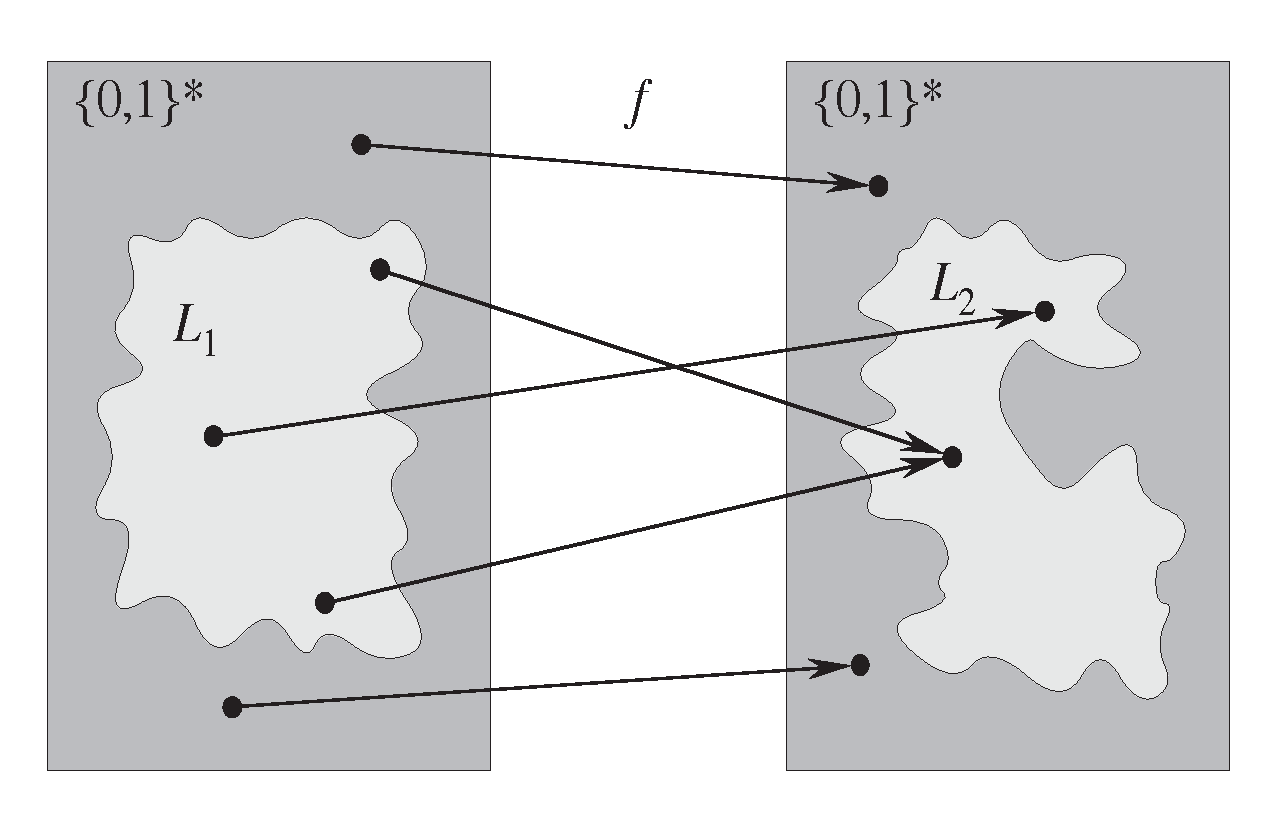
\includegraphics[height = 72pt]{reduction}
\end{centering}
\begin{itemize}
  \item To show decision problem $L_2$ is NP-complete, find an NP-complete problem $L_1$.
  \item Let $x$ be a binary encoding for some input to problem $L_1$.
  \item Give a polynomial-time algorithm $f$ to convert all instances of $L_1$ into an instance of $L_2$ such that for all strings $x$, $x \in L_1 \Leftrightarrow f(x) \in L_2$.
\end{itemize}
\end{frame}

\section{Definitions}

\begin{frame}
\frametitle{The definition of 3SAT}
\begin{itemize}
  \item Let $C = {c_1, \ldots, c_m}$ be a set of clauses on a finite set of $U$ boolean variables 
  \item A \emph{clause} is a disjunction of three literals.
  \begin{itemize}
    \item Given a variable $u$, a \emph{literal} is either $u$ or $\neg u$. If $u = T$, then $\neg u = F$.
    \item Example clause: $(\neg u_2 \lor u_3 \lor \neg u_4)$.
  \end{itemize}
  \item $C$ is \emph{satisfiable} $\Leftrightarrow$ there exists some truth assignment for $U$ that satisfies each clause in $C$.
  \item 3SAT returns {\sc yes} if $C$ is satisfiable and {\sc no} otherwise.
\end{itemize}
\end{frame}

\begin{frame}
\frametitle{The definition of a Bayesian network}
A \emph{Bayesian network} is a tuple $(V, A, P)$ where $V$ is a set of variables (vertices), $A$ is a set of arcs (edges), and $P$ is a set of conditional probability tables, one for each vertex.
\end{frame}

\begin{frame}
\frametitle{Bayesian network inference as decision problem}
\begin{itemize}
  \item Inference (IBN; inference in Bayesian network) is a computation problem. We need a decision problem to do the reduction.
  \item Define IBND (IBN decision) to
  \begin{itemize}
    \item Return {\sc yes} if $P(Y = T) > 0$
    \item Return {\sc no} otherwise.
  \end{itemize}
  \item Clearly $\text{IBND} \leq \text{IBN}$: if we had a solver for IBN, we simply compare the output to 0 as above to get a solver for IBND.
  \item \emph{Conversely, if we show IBND is NP-complete, then IBN must also be NP-complete.}
\end{itemize}
\end{frame}

\section{Reduction}
\begin{frame}
\frametitle{Constructing a Bayesian network from 3SAT, overview}
\includegraphics[width=\textwidth]{proof}
\end{frame}

\begin{frame}
\frametitle{Constructing a Bayesian network from 3SAT}
\begin{itemize}
  \item A \emph{truth setting component} adds one node $u_i$ for each boolean variable in $U$ and sets $p(u_i = T) = \frac{1}{2}$.
  \item A \emph{clause-satisfaction-testing subcomponent} adds one node $C_j$ for each clause and drawns an arc from edge variable to its clause. $p(C_j = T | \pi_{C_j}) = 1$ if and only if $C_j$ is satisfied.
  \begin{itemize}
    \item Consider (again) $C_j = (\neg u_2 \lor u_3 \lor \neg u_4)$.
    \item $p(C_j = T | u_2 = T, u_3 = F, u_4 = F) = 1$
    \item $p(C_j = T | u_2 = T, u_3 = F, u_4 = T) = 0$.
  \end{itemize}
  \item An \emph{overall-satisfaction-testing component} adds one node $D_j$ for each clause and adds the arcs $(C_j, D_j)$ and $(D_{j-1}, D_j)$. $p(D_j = T | \pi_{D_j}) = 1$ if and only if all of its parents are $T$.
  \item Define $D_n = Y$. Then equivalently, $P(Y = T | C_1, \ldots, C_m) = 1$ if and only if each $C_j = T$. \emph{For the rest of the proof, we ignore the $D_j$.}
\end{itemize}
\end{frame}

\section{Proof}
\begin{frame}
\frametitle{$C$ is satisfiable $\Rightarrow p(Y = T) > 0$, part 1}
\begin{itemize}
  \item We want $P(Y)$, but the graph defines $P(Y, C_1, \ldots, C_m, u_1, \ldots, u_n)$
  \item So define $\alpha$ and $\beta$ to be binary strings representing particular instantiations of $u_1, \ldots, u_n$ and $C_1, \ldots, C_m$. 
  \begin{itemize}
    \item E.g. $\alpha = 5 = 0101 \Rightarrow u_1 = F, u_2 = T, u_3 = F, u_4 = T$.
    \item Enumerating $\alpha$ and $\beta$ enumerates each assignment of the variables.
  \end{itemize}
  \item For notation, define $U_{\alpha} = \left\{ u_i = \alpha_{i} | 1 \leq i \leq n \right\}$ and $C_{\beta}$ similarly.
  \item We can then marginalize the $C_j$ and the $u_i$: $$p(Y = T) = \sum_{\alpha = 0}^{2^n - 1} \sum_{\beta = 0}^{2^m - 1} p(Y = T | C_{\beta}) p(C_{\beta} | U_{\alpha}) p(U_{\alpha})$$
\end{itemize}
\end{frame}

\begin{frame}
\frametitle{$C$ is satisfiable $\Rightarrow p(Y = T) > 0$, part 2}
\begin{itemize}
  \item If $C$ is satisfiable, then there exists a satisfying assignment $U_s$.
  \item This results in clause assignment $C_1$, i.e. $c_i = T$ for $1 \leq i \leq m$, and appears a term in the sum, so $$p(Y = T) \geq p(Y = T | C_1) p(C_1 | U_s) p (U_s).$$
  \item Show each term is $> 0$:
  \begin{itemize}
    \item Since $C_1$ satisfies each clause, $p(Y = T | C_1) = 1$.
    \item By construction, $p(U_s) = \left( \frac{1}{2} \right)^n$.
    \item Since $U_s$ satisfies each clause, $p(C_s | U_s) = 1$ by construction.
  \end{itemize}
  \item Thus $p(Y = T) > 0$. $\Box$
\end{itemize}
\end{frame}

\begin{frame}
\frametitle{$p(Y = T) > 0 \Rightarrow C$ is satisfiable}
\begin{itemize}
  \item Prove the contrapositive: suppose $C$ is not satisfiable.
  \item Then for any truth assignment $U_{\alpha}$, some clause $c_j$ is not satisfied. Thus $p(C_1 = T | U_{\alpha}) = 0$, so $p$
  \item So any nonzero term in the sum must have $\beta \neq 1$.
  \item But if $\beta \neq 1$, we have $p(Y = T | C_{\beta}) = 0$.
  \item So each term is 0, so $p(Y = T) = 0$.
\end{itemize}
\end{frame}

\begin{frame}
\frametitle{The form of our constructed network provides strong corollaries}
\begin{itemize}
  \item Each node has indegree no larger than 3 (conditioned on more than 3 variables) $\Rightarrow$ even graphs of simple topology are intractable.
  \item Planar 3SAT is NP-hard, so even planar bipartite belief networks are NP-hard.
  \item \emph{Arguably, our construction relies on probabilities of 0 or 1 in the $C_j$ and $D_j$, so is a pathological case. Real-world cases are unlikely to resemble this reduction.}
\end{itemize}
\end{frame}
\end{document}

